% Created 2018-09-07 Fri 21:17
\documentclass[11pt]{article}
\usepackage[utf8]{inputenc}
\usepackage[T1]{fontenc}
\usepackage{fixltx2e}
\usepackage{graphicx}
\usepackage{grffile}
\usepackage{longtable}
\usepackage{wrapfig}
\usepackage{rotating}
\usepackage[normalem]{ulem}
\usepackage{amsmath}
\usepackage{textcomp}
\usepackage{amssymb}
\usepackage{capt-of}
\usepackage{hyperref}
\author{Eissa Nematollahi}
\date{2018-09-02}
\title{Machine Learning: Basic Workflow\\\medskip
\large Better understanding of the basic workflow in machine learning tasks}
\hypersetup{
 pdfauthor={Eissa Nematollahi},
 pdftitle={Machine Learning: Basic Workflow},
 pdfkeywords={},
 pdfsubject={},
 pdfcreator={Emacs 24.5.1 (Org mode 8.3.1)}, 
 pdflang={English}}
\begin{document}

\maketitle
\tableofcontents
\clearpage 

\section{Introduction}
\label{sec:orgheadline1}
Machine learning is a statistical approach for making data-driven decisions through building models that are capable of capturing some patterns in data. Using historical data, models are \emph{trained} to \emph{learn} some patterns expected to exist in unseen data as well. Such machine learning models can answer questions of the following types:
\begin{itemize}
\item Is a transaction fraudulent? (classification)
\item Is an email spam? (classification)
\item Does a patient have cancer? What is the confidence level of our decision? (classification)
\item How much demand for a product is expected in a particular day? (regression)
\item Does a group of news belong to the same category? (clustering)
\item Are beer and diaper bought together frequently? (association rules)
\end{itemize}
In addition, machine learning models can be trained to perform complex tasks, including:
\begin{itemize}
\item Driving a car (self-driving cars)
\item Recognizing zip-codes from the images of hand-written postal envelopes
\item Describing details of a photo
\end{itemize}

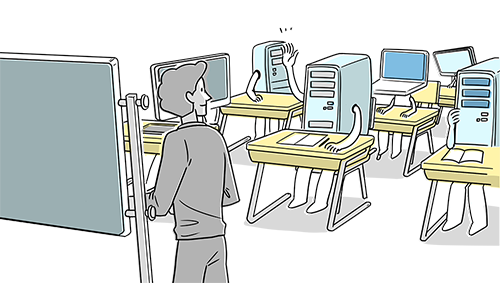
\includegraphics[width=.9\linewidth]{./images/machine-learning.png}


The following diagram depicts a common approach to building machine learning models. This workflow is explained in more details next.

\begin{figure}[htb]
\centering
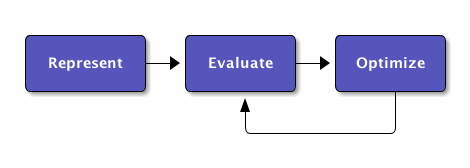
\includegraphics[width=.9\linewidth]{./images/machine-learning-workflow.png}
\caption{\label{fig:orgparagraph2}
Basic workflow in building machine learning models}
\end{figure}

\begin{enumerate}
\item We collect data and prepare them as input to machine learning algorithms. We require a
\begin{itemize}
\item \textbf{Training} data-set to train models.
\item \textbf{Validation} data-set to assess the trained models.
\item \textbf{Test} data-set to compute the prediction error of the best model.
\end{itemize}
\item We select a class of machine learning models, such as linear or logistic regression. These models are typically parametric whose parameters must be estimated on a training data-set. Model parameters estimation is formulated as one of the following optimization problems:
\begin{itemize}
\item \textbf{Maximum-likelihood estimation (MLE)} which maximizes the likelihood of data given model parameters.
\item \textbf{Maximum-aposteriori (MAP)} estimation which maximizes posterior probabilities given prior probabilities of the model parameters.
\item \textbf{Minimum total risk} which minimizes the empirical total risk, defined based on a proper loss function.
\end{itemize}
These optimization problems can be solved using optimization algorithms, such as the gradient descent method.
\item Machine learning models typically have a \textbf{complexity parameter}, which needs to be optimized for generalizability. For example, in the ridge regression (see \hyperref[orgtarget1]{Regression} section), the multiplier \(\lambda\) of the regularization term is the complexity parameter. In \(k\)-nearest neighbors, the \(k\) is the complexity parameter of the model. In this step, we tune the complexity parameter to obtain the best prediction error on the test data-set. For this, we may require to repeat steps (2) and (3) multiple times.
\end{enumerate}

In summary, a training data-set is used to train and build models. A validation data-set is used to evaluate the prediction power of the models, while tuning their parameters to generalize well on unseen data. Finally, a test data-set is used to compute the performance or the prediction power of the selected model.

\section{Machine Learning Models}
\label{sec:orgheadline2}
Machine learning algorithms look for hidden patterns in historical data with the \emph{hope} that the patterns will appear in future unseen data. Machine learning models, or \emph{learners}, are then built to capture the patterns and enable us to answer questions of interest by applying the models to unseen data. 

In machine learning, a data-set is typically a set of \textbf{records}, each containing a set of \textbf{features}. For example, in a clinical study, a record may represent information of a patient, while a feature may represent blood pressure of the patient. Some sample data-sets can be downloaded from \href{https://archive.ics.uci.edu/ml/index.php}{UCI Machine Learning Repository}. Popular machine learning libraries, such as scikit-learn in Python, provide APIs for loading popular data-sets.

Feature values can be \textbf{scalar}, \textbf{categorical}, \textbf{ordinal}, or \textbf{text}. 
\begin{itemize}
\item Scalar features typically contain measurement values, such as price, age, height, blood pressure, etc.
\item Categorical features hold categories from a finit (and typically small) set. For example, spam filtering data may have a \emph{Spam} feature with values \{YES, NO\} to indicate whether or not an email (a record of spam data) is spam.
\item Ordinal features are the same as categorical features in which categories are ordered. For example, T-shirt sizes may consist of the values \{SMALL, MEDIUM, LARGE\} which are obviously ordered.
\item Text features may hold any data in the text format, such as name, address, date, etc.
\end{itemize}

Machine learning algorithms include two major categories: supervised and unsupervised.

In \textbf{supervised} learning, there is an outcome feature, beside others, which is typically categorical or scalar. The goal is to predict the value of the outcome feature given the values of other features. The values of the outcome feature are given for historical data to \emph{supervise} training of the prediction models or learners. For example, given a set of emails, we can manually categorize them as spam or not-spam. Then, we build a model using some features of the emails along with their outcome values (spam/not-spam). The model can finally be used to predict whether a new email is spam or not. This problem is a typical example of the \emph{binary classification} problem. Other types include the \emph{regression problem} and the \emph{multi-class classification problem}.

In \textbf{unsupervised} learning, there is no outcome feature, and the objective is to find hidden relations among records. For example, given a set of news, we may want to know how to organize them into a few clusters. This is referred to as the \emph{clustering problem}. As another example, suppose that we are given a set of transactions in a store and would like to discover subsets of items that are bought together. This problem is referred to as the \emph{market basket analysis} or \emph{association rules}.

In the next section, we will see how to formulate the supervised learning problem as an optimization model. You may skip the theory and mathematics and jump to Section \hyperref[orgtarget2]{Bias-Variance Tradeoff}.

\section{Best Prediction Model}
\label{sec:orgheadline6}

\textbf{Note:} This section discusses how to formulate a supervised learning problem as an optimization model. Readers who would like to understand the concept without getting deeper in the theory and mathematics may skip this section.

A supervised machine learning problem (whether classification or regression) is to find the best parametric function, a.k.a \emph{model}, that reliably predicts target values of unseen data. To estimate model parameters, we may use maximum-likelihood or maximum-aposteriori estimation. Another common approach is to estimate model parameters by minimizing a loss function that measures the prediction error. We will see that these two approaches are indeed equivalent.

A machine learning problem can thus be cast as an optimization problem to find model parameters that minimize total loss or maximizes likelihood or posterior probabilities. Note that we build a model using training data-sets, thus called training a model, but compare models on test data-sets to see how they can generalize to unseen data. Model accuracy and generalizability are both important and will be discussed in more details in the next section.

To formulate the optimization problem, we need a set of records and a parametric function to approximate the true predictor, described mathematically as follows:
\begin{itemize}
\item A set of records \(\{(\boldsymbol{x}_i, y_i): i=1,2,\ldots,m\}\), in which \(\boldsymbol{x}_i=(x_{i1},\ldots,x_{in})\) is the input features and \(y_i\) is the target value; see Table \ref{tab:orgtable1}.
\item A parametric function \(f_{\boldsymbol{w}}(\boldsymbol{x})\) which maps a record \(\boldsymbol{x}\) from the input space to a value \(y\) in the target space.
\end{itemize}

\begin{table}[htb]
\caption{\label{tab:orgtable1}
Data table}
\centering
\begin{tabular}{ll}
\(\boldsymbol{X}\) & \(\boldsymbol{y}\)\\
\hline
\(x_{11}\quad x_{12}\quad \dots \quad x_{1n}\) & \(y_1\)\\
\(\vdots\quad\quad \vdots\qquad\qquad \vdots\) & \(\vdots\)\\
\(x_{m1}\quad x_{m2}\quad \dots \quad x_{mn}\) & \(y_m\)\\
\end{tabular}
\end{table}

To find unknown parameters \(\boldsymbol{w}\) using \textbf{maximum-likelihood estimation (MLE)} approach, we maximize \(p(\boldsymbol{X},\boldsymbol{y}|\boldsymbol{w})\), the likelihood of the input data given model parameters. Assuming that the input data are i.i.d. (independent and identically distributed), we have \(p(\boldsymbol{X},\boldsymbol{y}|\boldsymbol{w})=\Pi_{i=1}^m p(\boldsymbol{x}_i,y_i|\boldsymbol{w})\). Therefore, the maximum-likelihood estimation is equivalent to the following maximization problem:
\[
  \max_{\boldsymbol{w}} \sum_{i=1}^m \log p(\boldsymbol{x}_i,y_i|\boldsymbol{w}).
\]
Note that we maximize the log likelihood instead of the likelihood itself. The reason is that while they both are theoretically equivalent, the log likelihood maximization yields a more tractable problem for optimization algorithms. 

The maximum-likelihood estimation often yields a complex predictor and results in over-fitting -- a concept discussed in the next section. It turns out that the \textbf{maximum aposteriori (MAP)} estimation approach, which maximizes posterior probabilities \(p(\boldsymbol{w}|\boldsymbol{X},\boldsymbol{y})\), yields simpler models because of incorporating prior knowledge of unknown parameters. From the Bayes rule, we have
\[
p(\boldsymbol{w}|\boldsymbol{X},\boldsymbol{y})=\frac{p(\boldsymbol{w})p(\boldsymbol{X},\boldsymbol{y}|\boldsymbol{w})}{p(\boldsymbol{X},\boldsymbol{y})}.
\]
Thus, maximizing posterior probabilities is equivalent to the following maximization problem:
\[ 
  \max_{\boldsymbol{w}} \sum_{i=1}^m \log p(\boldsymbol{x}_i,y_i|\boldsymbol{w})+\log p(\boldsymbol{w}).
\]
Note that the objective of the MAP approach differs from that of the MLE approach in the term \(\log p(\boldsymbol{w})\). It turns out that this terms regularizes the solution by limiting the growth of the components of \(\boldsymbol{w}\). Addition of the regularization term results in simpler models and prevents over-fitting. 

\subsection{\label{orgtarget1} Regression}
\label{sec:orgheadline3}
The target values \(y_i\) in the regression problem are scalar, representing features such as weight, height, price, etc. Scalar target values may also be referred as the response values.

The \textbf{linear regression model} is one of the well-studied and popular machine learning models. In linear regression, we use the parametric function \(f_{\boldsymbol{w}}(\boldsymbol{x_i})=\boldsymbol{w}^T\boldsymbol{x_i}\) as the predictor. We assume that the target (response) values \(y_i\) contain Gaussian noise \(\epsilon\), .i.e.,
\[
  y_i = \boldsymbol{w}^T\boldsymbol{x_i} + \epsilon,\qquad \epsilon \sim N(0,\sigma^2).
\]
We can show that the maximum-likelihood estimation (MLE) is equivalent to the following maximization problem:
\[
  \max_{\boldsymbol{w}} -\frac{1}{2\sigma^2}\sum_{i=1}^m (y_i-\boldsymbol{w}^T\boldsymbol{x}_i)^2,
\]
which is a weighted \emph{sum of squared errors (SSE)} term.

In the maximum-aposteriori (MAP) approach, we assume that prior probabilities are Gaussian with \(\boldsymbol{w}\sim N(\boldsymbol{0}, \lambda^{-1}\boldsymbol{I})\). We can similarly show that the MAP estimation is equivalent to the following maximization problem:
\[
  \max_{\boldsymbol{w}} -\frac{1}{2\sigma^2}\sum_{i=1}^m (y_i-\boldsymbol{w}^T\boldsymbol{x}_i)^2 - \frac{\lambda}{2}\|\boldsymbol{w}\|_2^2,
\]
whose objective function is known as the \emph{ridge regression} model. The second (regularization) term guarantees that the parameters of the predictor are small enough to yield a simple model and prevent over-fitting.

The regression task is to first find \(\boldsymbol{w}\) that maximizes posterior probabilities. Then, use the predictor \(f_{\boldsymbol{w}}(\boldsymbol{x_i})=\boldsymbol{w}^T\boldsymbol{x_i}\) to estimate target (response) values of unseen data.

Although there is a closed form solution for the maximization problem, it is efficient to use iterative methods such as the \emph{gradient descent} algorithm.

\subsection{Classification}
\label{sec:orgheadline4}
In classification, target values are categorical and taken from a finite (and small) set of categories. The number of categories must be at least two. Classification problems with two categories are referred to as the binary classification problems. Most classification algorithm are developed for the binary case, since multi-class classification problems can be converted to a series of binary classification problems. 

The \textbf{generalized linear model (GLM)} extends the linear regression by applying a \emph{link function} to the response values. Thus, the predictor of the GLM is given by \(f_{\boldsymbol{w}}(\boldsymbol{x}_i)=g(\boldsymbol{w}^T\boldsymbol{x}_i)\), where \(g\) is a link function. Unlike the linear regression, which is not suitable for the classification problems, we can use GLM with proper link functions for classification tasks. 

The \textbf{logistic regression model}, which is widely used for the binary classification task, is an example of GLM, with \emph{sigmoid} function \(g(z)=1/(1+e^{-z})\) as its link function. Consider the binary classification problem and, without loss of generality, assume that \(y_i\in\{-1,1\}\). Thus, the predictor in the logistic regression is  
\begin{align*}
  f_{\boldsymbol{w}}(\boldsymbol{x}_i)=\frac{1}{1+e^{-\boldsymbol{w}^T\boldsymbol{x}_i}},
\end{align*}
whose value is interpreted as the probability of having \(y_i=1\) given \(\boldsymbol{x}_i\). In other words, we have
\begin{align*}
p(y_i=y|\boldsymbol{x}_i) &= \frac{1}{1+e^{-y\boldsymbol{w}^T\boldsymbol{x}_i}},\qquad y\in\{-1,1\}.
\end{align*}
It is easy to verify that \(p(y_i=-1|\boldsymbol{x}_i) + p(y_i=1|\boldsymbol{x}_i) = 1\). We observe that the Bernoulli model can describe the outcome of the target value with the latter probabilities. Thus, assuming that the records are i.i.d., we can show that the maximum-aposteriori estimation of \(\boldsymbol{w}\) can be obtained by solving the following optimization problem:
\[
\max_{\boldsymbol{w}} -\sum_{i=1}^m \log(1+e^{-y_i\boldsymbol{w}^T\boldsymbol{x}_i}) -\frac{\lambda}{2}\|\boldsymbol{w}\|_2^2.
\]
As noted previously, the gradient descent algorithm can be used to solve the latter optimization problem and obtain the unknown vector \(\boldsymbol{w},\) which defines the predictor model. The predictor can then be used to compute the posterior probabilities of unseen records. Of course, label \(y\) of an unseen record \(\boldsymbol{x}\) can be easily computed from its posterior probabilities:
\[
  y(x)=\begin{cases}
          1\quad f_{\boldsymbol{w}}(\boldsymbol{x}) \ge 0.5,\\
          0\quad \text{otherwise.}
         \end{cases}
\] 

\subsection{Summary}
\label{sec:orgheadline5}
In summary, we saw that machine learning problems can be cast as optimization models. To formulate the optimization model, we need a set of records (training data-set), a parametric function (model), and a measure to find best model parameters. For example, likelihood of data given parameters may be maximized to yield maximum-likelihood estimation (MLE) of the model parameters. Alternatively, posterior probabilities may be maximized to yield maximum-aposteriori (MAP) estimation of the parameters. 

The MAP estimation results in an optimization problem whose optimal solution yields models with an adjustable complexity parameter \(\lambda\). As the model complexity increases, the prediction error on training data-sets is expected to decrease. Although very accurate on training data-sets, highly complex models are not generalizable to unseen data. Thus, there is a tradeoff between accuracy and generalizability of a model. In the next section, we will learn more about this tradeoff and characteristics of a good model.

\section{\label{orgtarget2} Bias-Variance Tradeoff}
\label{sec:orgheadline7}
As we discussed in the previous section, the prediction error on training data-sets is not enough to assess the goodness of a model. A good model needs to be generalizable to unseen data as well. It can be shown that the expected error of a model is composed of three terms: \emph{bias}, \emph{variance}, and an irreducible error term; consult with \href{https://web.stanford.edu/~hastie/ElemStatLearn/}{The Elements of Statistical Learning} for the proof and detailed discussion.

Bias is an error term that measures the \textbf{accuracy} of a model. High bias means that the model does not really capture hidden patterns in the data. This is referred to as \textbf{under-fitting}. We ideally want a low bias model; but how low should the bias be? Models with a very low bias tend to capture the noise in the training data-set, resulting in an \textbf{over-fitted} model. Therefore, the bias itself as a measure is not enough for building a good model; we need another measure.

The variance is an error term that measures the \textbf{consistency} of a model. Over-fitted models usually have high variance. A high variance indicates that the model is not generalizable to unseen data.

Ideally, we want a model that captures hidden patterns in the training data-set (low bias) and generalizes well to unseen data (low variance). Thus, we need to minimize both bias and variance, simultaneously. As shown in Figure \ref{fig:orgparagraph3}, a simple model usually has a high bias; such a model is under-fitted, regardless of having low or high variance. Assuming that we have enough training data-set, increasing model complexity will cause the bias and variance to decrease until a point where the variance will begin to grow. That point defines a model with optimal complexity that minimizes both bias and variance, simultaneously.

\begin{figure}[htb]
\centering
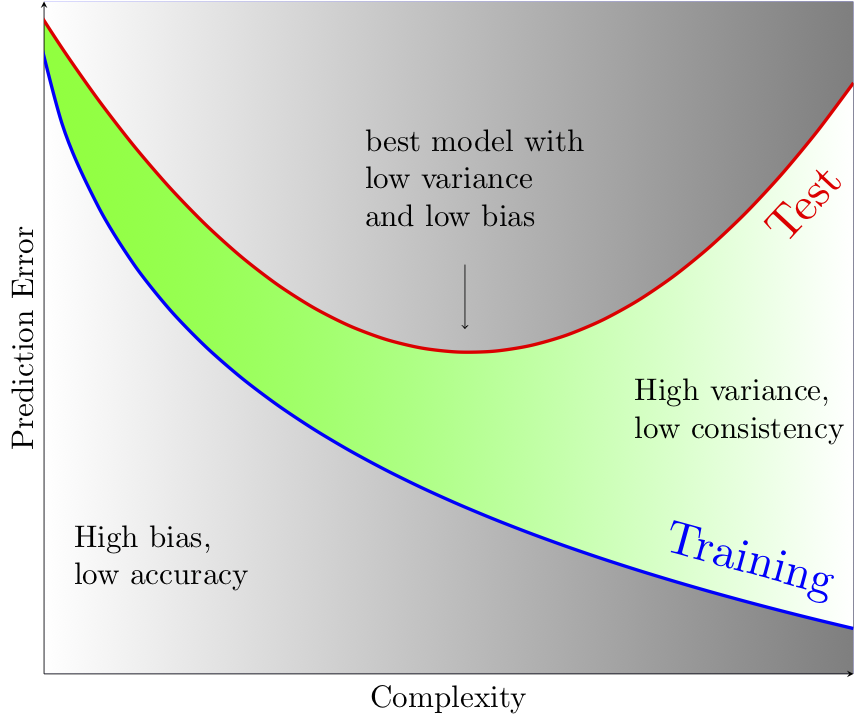
\includegraphics[width=.9\linewidth]{./images/bias-variance-tradeoff.png}
\caption{\label{fig:orgparagraph3}
Bias-variance tradeoff in machine learning: A simple model yields high bias (low accuracy) on both training and test data-sets. A complex model, on the other hand, yields high variance (low consistency) as it captures noise in the training data-set, too.}
\end{figure}

In summary, we have the following four cases, as depicted in Figure \ref{fig:orgparagraph4}:
\begin{itemize}
\item Both bias and variance are high. The model is both inaccurate and inconsistent: under-fitted model. Typically, this occurs when there is no enough training data. To avoid this case, we simply collect more data.
\item Variance is low while bias is high: The model is consistent but inaccurate: under-fitted model.
\item Bias is low while variance is high: The model is accurate but inconsistent: over-fitted model.
\item Both bias and variance are low: The model is both accurate and consistent: well-fitted model.
\end{itemize}

\begin{figure}[htb]
\centering
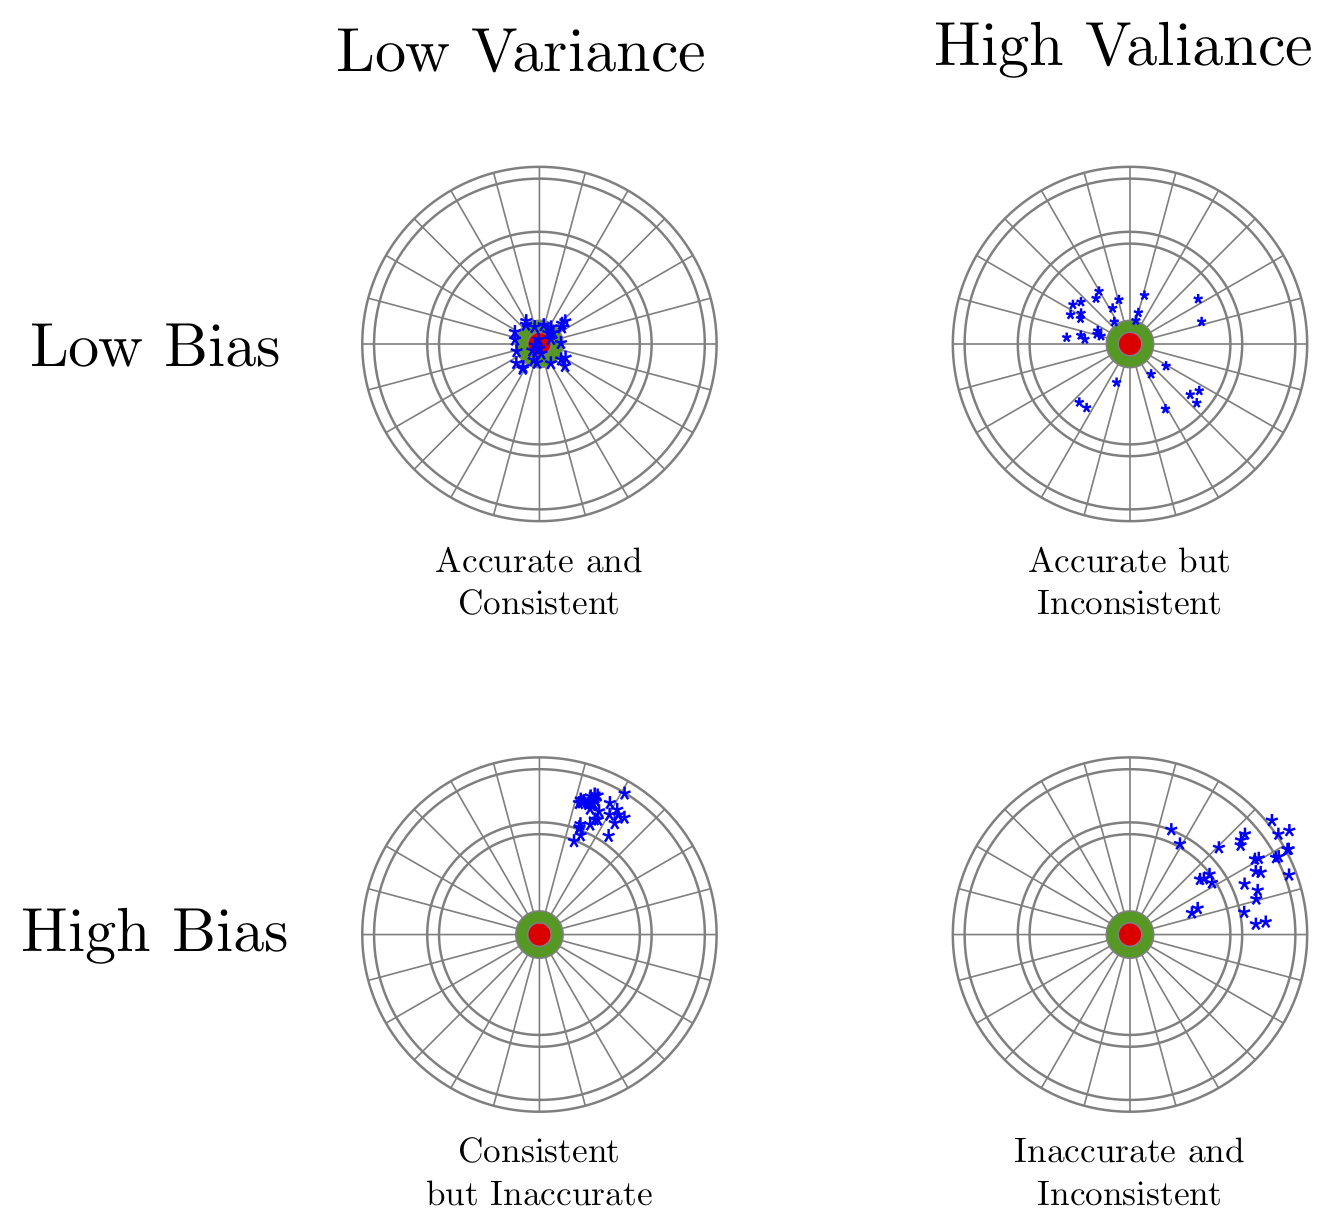
\includegraphics[width=.9\linewidth]{./images/bias-variance-dart.png}
\caption{\label{fig:orgparagraph4}
Bias-variance variation: A good model has both low bias and low variance. High bias indicates that the model in under-fitted, and high variance signals that the model is over-fitted.}
\end{figure}

So far we learned that a good model, trained on the training data-set, has a low prediction error on the test data-set. However, we cannot rely on one set of training and test data, as we may get lucky to obtain low prediction error on one test data-set. In other words, one set of data is not representative of the whole space of possible unseen data. 

One solution is to collect many sample data and repeat the process to compute prediction errors and combine them to obtain a good estimate of the true prediction error of the model. One way to combine the prediction errors is to take the average of them.

The problem with the latter solution is that we may not be able to collect many sets of data. Cross-validation technique, discussed in the next section, is a well-known approach to generate multiple sets of training and test data-sets from a single data-set.

\section{Cross-Validation}
\label{sec:orgheadline9}
One of the most widely-used methods to estimate the prediction error of a machine learning model is the \emph{\(K\)-fold cross-validation}. The cross-validation technique is not meant to be used for model building; its purpose is merely to obtain more accurate estimate of the prediction error of a given model. The method \emph{randomly} partitions data into \(K\) folds (or parts) and generates \(K\) splits of training-test data-sets as follows: for each \(k\in\{1,2,\ldots,K\}\), the \(k\)-th fold in split \(k\) is the test data-set, while the rest forms the training data-set. A five-fold cross-validation data-partitioning is depicted in the following diagram.

\begin{figure}[htb]
\centering
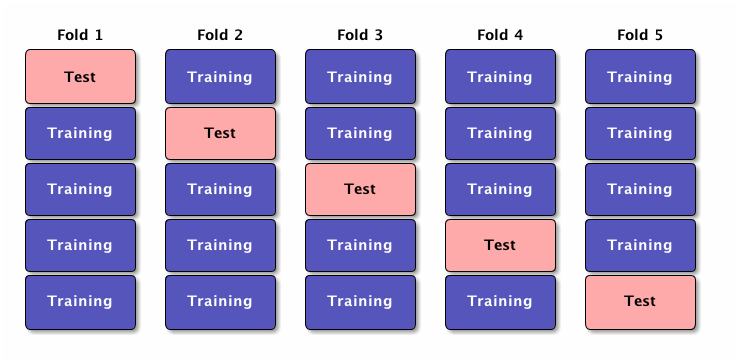
\includegraphics[width=.9\linewidth]{./images/cross-validation.png}
\caption{\label{fig:orgparagraph5}
Five-fold cross-validation}
\end{figure}

Simple random sampling may be used for partitioning the data-set into \(K\) folds. However, to have proportional distribution of the records in both training and test data-sets, we can employ stratified sampling.

After generating \(K\) sets of data, we build models on the training data-sets and compute the prediction errors on the test data-sets. The prediction error of a machine learning algorithm is then computed by combining all the computed prediction errors. For example, we can compute the average of the computed errors as the ultimate prediction error.

\subsection{Choice of \(K\)}
\label{sec:orgheadline8}
A version of the cross-validation is the \textbf{leave-one-out} or \(m\)-fold cross-validation approach, where \(m\) is the number of records in the training data-set. Therefore, in each fold, there is only one record for the test data-set, while the rest of the records are used for training the model. The leave-one-out approach is relatively expensive and yields a low bias, high variance prediction error.

As \(K\) decreases, both the number of data-sets (folds) and the size of each training data-set shrink while the test data-set expands. It means that the amount of computation decreases since there are fewer models to train. Nevertheless, the prediction errors are expected to have higher bias and lower variance. The optimal choice of \(K\) is problem dependent; however, \(K=5\) and \(K=10\) are commonly used values in practice.
\end{document}